\documentclass[pdftex,10pt,a4paper]{article}
\title{\textbf{Kidney Morphogenesis Cellular Automaton - Model Details}\newline }
\author{Ben Lambert}
\usepackage[authoryear]{natbib}
\usepackage[titletoc,toc]{appendix}
\usepackage[pdftex]{graphicx}
\usepackage{url,times}
\usepackage{graphicx}
\usepackage{epstopdf}
\usepackage{amsmath}
\usepackage[all]{xy}
\usepackage{pxfonts}
\usepackage{colortbl}
\usepackage{color}
\usepackage{subfigure}
\usepackage{gensymb}
\usepackage{ctable}
\usepackage[justification=centering]{caption}[2007/12/23]
\usepackage{longtable}
\usepackage{pst-func}
\usepackage{pst-math}
\setlength{\parindent}{0.0in}
\setlength{\parskip}{0.1in}
\usepackage[margin=0.5in]{geometry}
\renewcommand{\bibname}{Works Cited}
\usepackage{listings}
\usepackage{setspace}
\usepackage{algorithm}
\usepackage{bbm}

\newcommand{\HRule}{\rule{\linewidth}{0.5mm}}
\begin{document}

\maketitle
\doublespacing
\section{Introduction}
The aim of this model is to recapitulate the development of the Uretic Bud \textit{in vivo} in 2D. However, it is also hoped that the model may be useful for the study of \textit{in vitro} explants. The details of the model are described in brief below:
\begin{itemize}
\item A 2 dimensional rectangular domain, where the points in the array represent the presence of:
\begin{itemize}
\item Epithelium cells - which consume GDNF
\item Metanephric mesenchymal cells (MM) - which produce GDNF
\item Extracellular matrix (ECM) - which allow for free diffusion of GDNF
\end{itemize}
\item Epithelium cells comprising either:
\begin{itemize}
\item A \textit{flat} membrane at the base of the simulation domain (aimed at recapitulating the \textit{in vivo} conditions from which the UB initially forms \textit{in utero}.)
\item A mass of epithelium cells with in general, curved boundaries, suspended towards the centre of the simulation domain (representative of the \textit{in vitro} explant experiment initial conditions.)
\end{itemize}
\item A diffuse collection of mesenchymal cells initially separate from the epithelium.
\end{itemize}

\section{GDNF field}
\subsection{Steady state reaction-diffusion equation}
Cells in the MM produce GDNF, and it diffuses freely across the ECM layer, and through the epithelium (being consumed by the latter). The reaction-diffusion type equation here will be assumed to be in equilibrium, since the diffusive timescale of GDNF is much less than that of the timescale of cell division. As such, the following is the form of the equation being solved:

\begin{equation}\label{eq:diffnorm}
D_G \nabla^2 = \Phi_G
\end{equation}

Where in (\ref{eq:diffnorm}) $D_G$ refers to the diffusion coefficient for GDNF, and $\Phi_G$ is the local rate of GDNF production or consumption (dependent on whether the cell in question is epithelium or mesenchyme). Specifically the rate of GDNF consumption is assumed to have the following form:

\begin{equation} \label{eq:production}
\Phi_G =\begin{cases}
K_G G, & \text{for epithelium}.\\
-\rho_G, & \text{for mesenchyme}.\\
0, & \text{for the extracellular matrix}.
\end{cases}
\end{equation}

It is assumed that the rate of GDNF consumption is linearly-dependent on the concentration of substrate. This assumption is likely violated when the GDNF concentration is high, and the cell Ret-receptors are saturated. In later versions of this model, it may be better to assume a Hill-type reaction rate. (Although it is unclear as to what range of concentrations of GDNF are likely to saturate the Ret receptors, and whether these are likely to be encountered either \textit{in vivo} or in experiments conducted thus far \textit{in vitro}.) However, this sort of non-linear consumption function is best handled by solving the parabolic time-dependent reaction-diffusion equation (see section \ref{subsec:timedependent}). It is assumed to begin with that the mesenchyme GDNF production rate is constant, partly for simplicity, although this will be relaxed in latter models which, for example, allow mesenchymal GDNF production rates to be a positive function of their proximity to epithelium cells (perhaps as a proxy for Wnt11 levels).

The equation in (\ref{eq:diffnorm}) is non-dimensionalised using the following transformations:
\begin{equation}\label{eq:difftrans1}
\eta = \frac{x}{\Delta}
\end{equation}

\begin{equation}\label{eq:difftrans2}
g = \frac{G}{G_x}
\end{equation}

Where in (\ref{eq:difftrans1}) $\Delta$ refers to the typical cell dimensions (approximated as 5 $\mu m$),and $G_x$ is the concentration of GDNF typically found \textit{in vivo} (a value is currently not assigned here, since it is not strictly necessary for the non-dimensionalised simulation). These transformations result in the following non-dimensional form of the steady-state reaction-diffusion equation:

\begin{equation}\label{eq:diff-dimensionless}
\nabla_\eta^2 g = \frac{\phi_g}{d_g}
\end{equation}

Where in (\ref{eq:diff-dimensionless}), $d_g = \frac{D_G}{K_G \Delta^2}$, $\phi_g = \frac{\Phi_G}{K_G G_x}$, and $\nabla_\eta^2$ is the laplacian in the non-dimensional $\eta$ spatial coordinates.

The boundary conditions which are assumed are: no-flux at the base of the Wolffian Duct and top of the simulation domain, and periodic boundary conditions at either width. A finite difference approximation is used, with the no-flux boundary conditions at the top and bottom of the domain represented by the following relations for the non-dimensional GDNF field:

\begin{align*}
g_{0,j}& = g_{1,j}\\
g_{M,j}& = g_{M+1,j}\\
\end{align*}

where this holds $\forall j = 1,...,N$. $M$ here is the depth of the simulation domain in terms of cell dimensions. Similarly, for the periodic boundary conditions:

\begin{align*}
g_{i,0}& = g_{i,N}\\
g_{i,N+1}& = g_{i,1}\\
\end{align*}

where this holds $\forall i = 1,...,M$. $N$ here is the width of the simulation domain in terms of cell dimensions.

The finite-difference approximation for solving the steady-state reaction-diffusion equation is hence of the form:

\begin{equation}\label{eq:finitediff}
g_{i+1,j} + g_{i-1,j} + g_{i,j+1} + g_{i,j-1} - (4 + \epsilon_{i,j})g_{i,j} = -\psi_{i,j}
\end{equation}

Where in (\ref{eq:finitediff}):
\begin{equation}
\epsilon_{i,j} =\begin{cases}
\frac{1}{d_g}, & \text{for epithelium}.\\
0, & \text{for mesenchyme}.\\
0, & \text{for the extracellular matrix}.
\end{cases}
\end{equation}

Also, in (\ref{eq:finitediff}):
\begin{equation} \label{eq:psi}
\psi_{i,j} =\begin{cases}
0, & \text{for epithelium}.\\
\frac{\gamma}{d_g}, & \text{for mesenchyme}.\\
0, & \text{for the extracellular matrix}.
\end{cases}
\end{equation}

Where in (\ref{eq:psi}), $\gamma = \frac{\rho_G}{K_G G_x}$ captures the relative rate of GDNF production by the mesenchyme compared to the rate of GDNF consumption by epithelium under normal cellular conditions. It is assumed that $\gamma = 1$ in the simulations, in the absence of information regarding the relative weight of these two mechanisms. The diffusion rate constant, $D_G$, is assumed to be 10 $\mu m^2 s^{-1}$ (following Menshykau and Iber). If we assume that the diffusive time scale is similar to that of the consumption rate of GDNF we find that:

\begin{equation}\label{eq:diffusiontime}
k_G \sim \frac{D_G}{\Delta_{domain}^2} 
\end{equation}

Where in (\ref{eq:diffusiontime}), $\Delta_{domain}$ refers to the simulation domain spacial dimensions. Typically, the simulation takes place in a domain with a width of 100 cells and a similar depth. This leads to an effective reaction rate constant of $k_G = 1 \times 10^{-5} s^{-1}$. This results in a dimensionless diffusion rate of $d_g = 4000$. Previously, without this approximation, the simulation was conducted using a value of $d_G = 200$; resulting in heterogeneous GDNF concentrations across the domain, with relatively low values in epithelial crypts. With this higher value of the effective diffusion rate however, the concentration is much more uniform, with low concentration gradients resulting. As a result, this higher value of the diffusion rate made it considerably harder to generate branching patterns.

In the simulation, it is assumed that the GDNF field does not vary significantly within a particular time step. As such (in order to improve computational speed), the GDNF field is only updated at the end of each time step, not after each cell movement or proliferation. Ultimately however, it will be important to test whether the model conclusions are sensitive to this assumption.

\subsection{Time-dependent reaction-diffusion numerical approximation}\label{subsec:timedependent}
This section specifies the details of the non-dimensionalisation of the reaction-diffusion equation to be used to study branching \emph{in vitro} of explanted kidney epithelium cells in a GDNF broth. Another reason for using a parabolic quasi-steady state reaction-diffusion equation is that it allows for easier inclusion of non-linear GDNF consumption/production functions than that for the elliptic case. Both explicit and implicit finite difference schemes are employed to numerically simulate the system.

\subsubsection{Details of the non-dimensionalisation}
The specific reaction-diffusion equation relevant to the epithelium-broth system is of the form:

\begin{equation}\label{eq:rd_time}
\frac{\partial G}{\partial t} = D_G \nabla^2 - \Phi_G
\end{equation}

Where in (\ref{eq:rd_time}) $D_G$ refers to the diffusion coefficient for GDNF, and $\Phi_G$ is the local rate of GDNF consumption which occurs at epithelium cells.


The equation in (\ref{eq:rd_time}) is non-dimensionalised using the following transformations:
\begin{equation}\label{eq:difftrans4}
\eta = \frac{x}{\Delta}
\end{equation}

\begin{equation}\label{eq:difftrans5}
g = \frac{G}{G_x}
\end{equation}

\begin{equation}\label{eq:difftrans6}
\tau = \frac{t}{T}
\end{equation}

Where in (\ref{eq:difftrans4}) $\Delta$ refers to the typical cell dimensions (approximated as 5 $\mu m$),and in (\ref{eq:difftrans5}), $G_x$ is the concentration of GDNF typically found \textit{in vivo} (a value is currently not assigned here, since it is not strictly necessary for the non-dimensionalised simulation). In (\ref{eq:difftrans6}), $T$ is the time scale of a typical cell division; assumed to be $T \sim 1 hr$. These transformations result in the following non-dimensional form of the time-dependent reaction-diffusion equation:

\begin{equation}\label{eq:nondenom}
\frac{\partial g}{\partial \tau} = d_g \nabla_\eta^2 g - \phi_g
\end{equation}

Where in (\ref{eq:nondenom}), $g = G/G_x$, $d_g = \frac{T D_G}{\Delta^2}$, and, $\phi_g = \frac{\Phi_G}{K_G G_x}$. Note here that, the dimensionless diffusive rate here represents the ratio of two time scales: the cell division time as compared to the diffusion time scale. The latter can be shown to be (for a diffusion rate of $D_G = 10 \mu m^2 s^{-1}$, and a cell dimension of $\Delta \sim 5 \mu m$) approximately of order $\frac{\Delta^2}{D_G} \sim 2.5 s$; resulting in an dimensionless diffusion rate of order $d_g \sim 1500 $.

The two ways considered to numerically simulate the system were \emph{explicit} and \emph{implicit} finite difference schemes. They numerically approximate (\ref{eq:nondenom}), by using the following schemes:

\begin{equation}\label{eq:explicit}
\mathbf{g^{t+1}} = \Delta_\tau [(d_g \nabla_\eta^2 + \frac{I_{MN}}{\Delta_\tau})\mathbf{g^t} - \mathbf{\Psi}(\mathbf{g^t})]
\end{equation}

\begin{equation}\label{eq:implicit}
\mathbf{g^{t+1}} = [I_{MN} - \Delta_\tau d_g \nabla^2]^{-1}(\mathbf{g^t} - \Delta_\tau \mathbf{\Psi}(\mathbf{g^t}))
\end{equation}

Where (\ref{eq:explicit}) refers to the \emph{explicit} scheme, and (\ref{eq:implicit}), to the \emph{implicit} one, and $\Delta_\tau$ is the time step taken. In (\ref{eq:explicit}) and (\ref{eq:implicit}), $\mathbf{\Psi}$ is a vector which contains all GDNF consumption and production terms, and can, in general, be a non-linear function of GDNF. It is assumed that $\mathbf{\Psi}$ is formed using the cell positions corresponding to the current (known) time period. Although this results in a somewhat 'bastardised' implicit scheme, it is perhaps a reasonable approximation, as cell positions are not likely to change significantly between the time steps taken, since the cell cycle is much longer that the typical GDNF consumption time. In (\ref{eq:implicit}) the RHS will be calculated using Matlab's inbuilt backslash operator to avoid the computational overhead of calculating the matrix inverse.

\section{Epithelium cell behaviour}
\subsection{Algorithm governing cellular behaviour}
In this section I describe the behaviours of the epithelium cells in the cellular automaton model. In the simulation, each epithelium cell is visited in a random order, (actually epithelium and mesenchyme are updated together, so the randomised order corresponds to both cell types), and updated at each discrete time step according to the following pseudo-algorithm:

\begin{itemize}
\item \textit{Available cells} - Are neighbouring cells available for movement or proliferation? If yes, proceed to step 2. If no, move on to next cell. Whether a cell is available depends on the specific rules in place (see section \ref{sec:rule_available} for more details).
\item \textit{Move or proliferate} - Draw a random number $X\sim unif(0,1)$. If $P_{move}>X$ then proceed to \textit{move}. If not, proceed to \textit{proliferate}.
\item \textit{Move} 
\begin{enumerate}
\item \textit{Calculate the probability that a move takes place, $P_m$} - Based on the specific rules in place calculate the probability that a move takes place (see section \ref{sec:rule_pmove} for more details).
\item \textit{Does a move take place?} - Draw a random number $X\sim unif(0,1)$. If $P_{m}>X$ then proceed to next step. Otherwise, consider next epithelium cell.
\item \textit{Calculate probability of moving to each of the available cells} - Based on the specific rules being used, calculate probabilities of moving to each of the available target cells (see section \ref{sec:rule_selection} for more details about the options for rules used here). 
\item \textit{Choose amongst the available cells in accordance to their probability and move the cell in question}.
\end{enumerate} 
\item \textit{Proliferate}
\begin{itemize}
\item The framework is exactly analogous to that of \textit{Move} detailed above. However, the rules chosen for proliferation or moving are allowed to be different in the simulation. In proliferation, the mechanism is slightly different due to the fact that a daughter cell is created in the target cell, rather than a cell simply moved there.
\end{itemize}
\item Consider next cell, returning to first step.
\end{itemize}

The program has been created in Matlab which allows for a number of permutations of the rules to be tried by the user. However, there are some combinations which are not allowed due to internal inconsistency amongst them. The idea is to allow the model's results to be easily tested for robustness to assumptions made.

\subsection{Rules governing whether neighbouring cells are available}\label{sec:rule_available}
In this section I will detail the various different rules which govern into which cells an active cell (the one being updated) can move or proliferate. These rules are allowed to be different for cells which are moving or proliferating.

\begin{enumerate}
\item \textit{Number of neighbours} - the choice here governs whether 4 (up, down, left, and right) or 8 (all points of a compass) are surveyed as potential candidates for a move or proliferation.
\item \textit{Connectivity of cells}
\begin{enumerate}
\item All vacant cells are allowed.
\item Moves or proliferations are allowed into vacant cells only if the active cell (the one being moved, or the daughter cell being created) are connected to other cells. Here connectivity means that there is at least one 4-neighbour (up, down, left or right) which is occupied by an epithelium cell. For a visual explanation of this, see figure \ref{fig:connected}. \label{item:sticky1}

\begin{figure}[t] 
\centering
\scalebox{0.5} 
{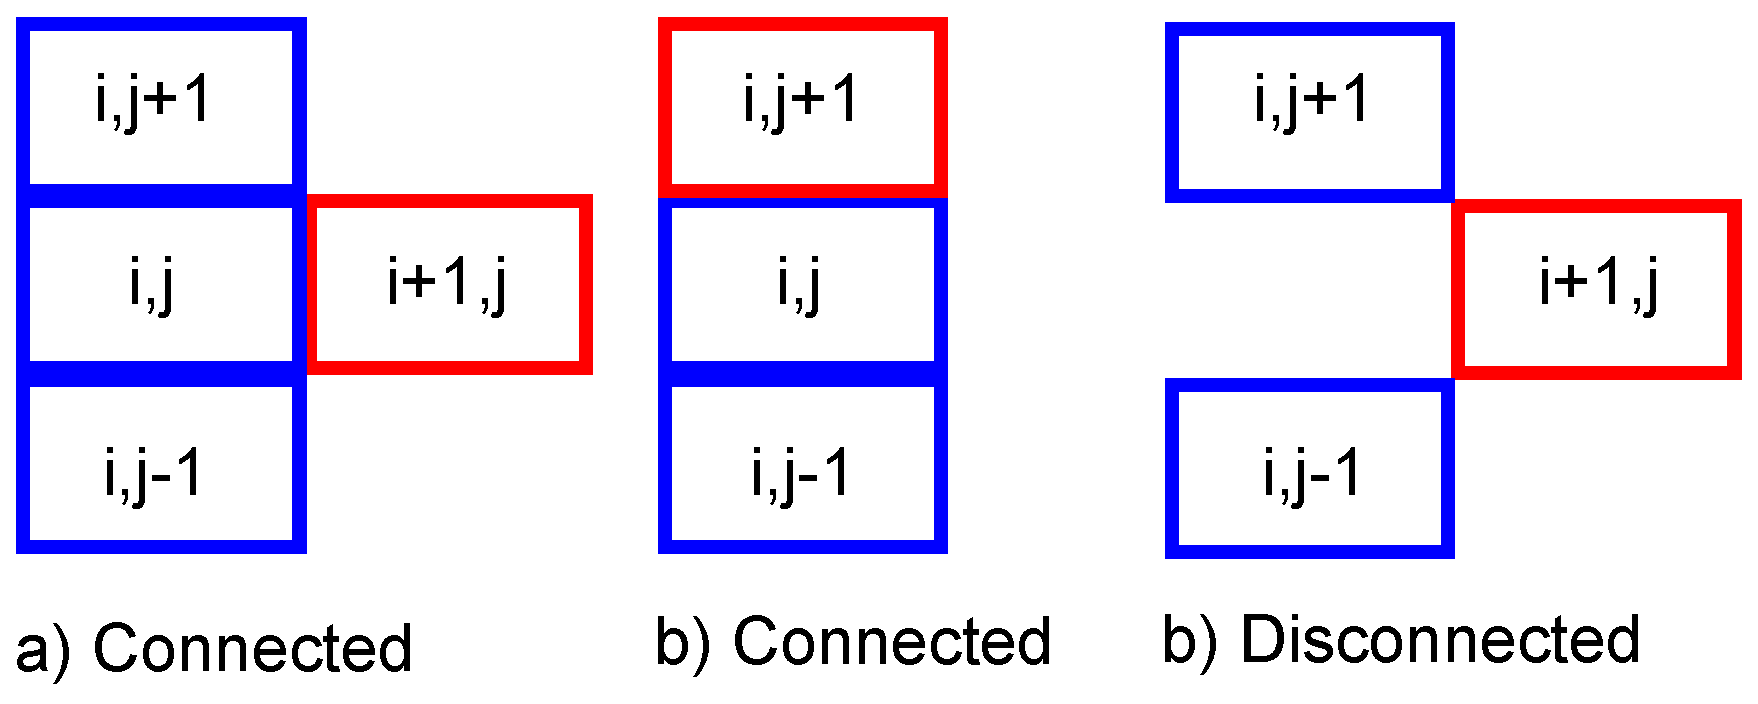
\includegraphics{connected.eps}}
\caption{An explanation of 'connectivity' for epithelium cells. All cells here are epithelium, the one highlighted in red is the cell which has been moved. The first two moves would be allowed, whereas the last is not.}\label{fig:connected}
\end{figure} 


\item Same as above, but more stringent. Only allow moves if all cells are connected. This allows for the possiblity of a move leaving one cell unconnected.\label{item:sticky2}
\item All vacant cells and mesenchyme are allowed as possible move/proliferation locations. If a movement into a cell occupied by a mesenchymal cell occurs, then the mesenchyme cell is removed from the simulation.\label{item:mes1}
\item Same as \ref{item:mes1}, although only allow movement into a space if that active cell remains connected. \label{item:sticky3}
\item Same as \ref{item:sticky3}, although instead of killing mesenchyme cell (upon movement into its space), move the mesenchyme into a vacant space neighbouring it (as shown in figure \ref{fig:8NN}). If there are no vacant spaces available for the mesenchyme cell to move into, then the move is not allowed. If multiple spaces are available for the mesenchyme to move into, then a space is chosen either at random or weighted towards the direction in which they were pushed (see section \ref{sec:weighted}).\label{item:sticky4}
\item Same as \ref{item:sticky4}, but prevent any epithelium movements if they lead to a mesenchyme becoming 'engulfed' by surrounding epithelium (see section \ref{sec:engulfment} for a further discussion).\label{item:sticky5}
\item Allow movements of epithelium into both vacant and mesenchyme grid locations (assuming the active cell is connected). However, allow mesenchyme to be moved non-locally (by non-local here I mean to a location which is not neighbouring) to a vacant location within a rectangular domain defined by the direction in which it was pushed. See section \ref{sec:nonlocal} for more details.\label{item:sticky6}
\end{enumerate}
\end{enumerate}


\begin{figure}[ht] 
\centering
\scalebox{0.5} 
{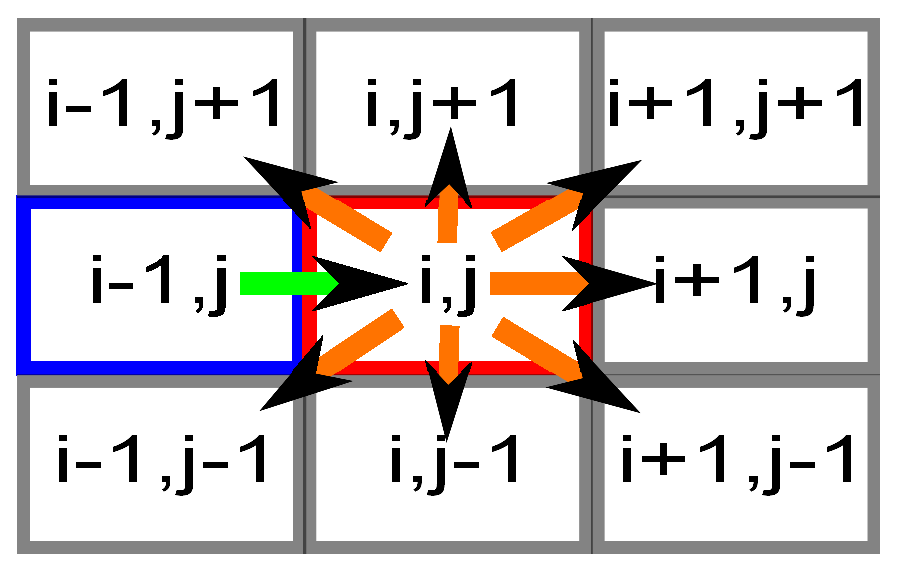
\includegraphics{8-NN.eps}}
\caption{The 7 available moves for a mesenchyme at $(i,j)$ after a epithelium at $(i-1,j)$ moves into its cell location. The grey cells are assumed to be vacant. Note that this epithelium move would not be allowed under certain rules as the active cell would become unconnected.}\label{fig:8NN}
\end{figure} 



The above rules \ref{item:sticky1}, \ref{item:sticky2}, \ref{item:sticky3}, \ref{item:sticky4}, \ref{item:sticky5} and \ref{item:sticky6} are phenomenlogical, but are aimed at mimicking the cell-cell adhesion experienced by the epithelium. Rules \ref{item:mes1}, \ref{item:sticky3}, \ref{item:sticky4}, \ref{item:sticky5}, and \ref{item:sticky6} are included as to allow an interaction between the epithelium cells and the mesenchyme, when the former move into the area occupied by the latter. It is thought that \ref{item:sticky4} is the most biologically realistic, since excess cell death is not typically observed, and cells do not 'jump' non-locally. However, there are issues with this particular framework, since it does not accommodate the ability of an incident epithelium layer to push on a dense layer of mesenchyme - an interaction which is observed in practice. This type of behaviour is not observed since there may not be any vacant spots for mesenchyme cells to move into in this single occupancy CA model. This motivated the introduction of non-local jumping of mesenchyme in schema \ref{item:sticky6} which is described in detail in section \ref{sec:nonlocal}. Rule \ref{item:sticky5} was introduced to investigate mechanisms which would prevent mesenchyme cells becoming isolated within an epithelium mass; which had occurred with the previous rules. A description of what is meant by 'engulfment' and the mechanism of operation for this rule are detailed in \ref{sec:engulfment}.

\subsection{Rules governing the calculation of $P_{m}$ or $P_p$ - the probability of a move or proliferation occurring after the action has been chosen}\label{sec:rule_pmove}
In this section I describe the available choices of model rules which govern the calculation of the probability of a move/proliferation occurring takes place. To be clear, this is the step after the choice has been made to either go down the algorithmic branches corresponding to \textit{Move} or \textit{Proliferate} respectively. It is chosen to make the decision as to whether to continue along each branch here, rather than at the stage before to allow for potentially different rules governing moving and proliferating respectively. The rules available for calculating whether or not a move/daughter cell creation takes place are given below:

\begin{enumerate}
\item The probability of a move/proliferation is a constant specified by the user.
\item The probability of a move/proliferation is a positive function of the local GDNF concentration (the level of GDNF for that cell at that grid point). The equation used here to specify the probability is that of a probit model 
\begin{equation}\label{eq:probit}
P(action) = \Phi(c_1 + c_2 g)
\end{equation}
Where in (\ref{eq:probit}), $\Phi$ is the standard normal CDF, and $action$ can either be a move or a proliferation event.\label{item:pmove_GDNF}
\item Move/proliferation probability is determined by the sum of all local positive GDNF gradients, between each of the available neighbours and the current location. Again, the model used here for the probability is the probit model:
\begin{equation}\label{eq:probit2}
P(action) = \Phi(c_1 + c_2 \sum\limits_{allowed}} (g^{neighbours} - g^{current})\times \mathbbm{1}(g^{neighbours} > g^{current})
\end{equation}
Where in (\ref{eq:probit2}), the indicator function $\mathbbm{1}(g^{neighbours} > g^{current})$, is equal to one if the gradient in GDNF allowed by the move is positive, and zero otherwise.\label{item:pmove_gradient}
\end{enumerate}

Rule \ref{item:pmove_GDNF} is aimed at allowing more cellular activity (moves or proliferations) in areas where GDNF concentration is higher. The use of a normal CDF here is partly to constrain the probability to lie in the appropriate (0,1) range, but can also act to provide thresholding-type behaviour, which may be necessary to generate discrete bud formation from the Wolffian Duct \textit{in vivo} opposed to a general 'swelling'. Rule \ref{item:pmove_gradient} allows more cellular activity in areas where there is more GDNF to be gained by a potential move or proliferation. I am less sure as to the biological realism of this latter rule, although for it could be thought of as a type of chemotaxis for moving cells, or orientated cell division for proliferating cells.

\subsection{Rules governing selection of move target or daughter cell location}\label{sec:rule_selection}
This last section on rules details how to determine the location (amongst the available, allowed neighbouring cells) into which either a cell should move or create a daughter cell. The rules governing how the probabilities of choosing a given target location are given below:

\begin{enumerate}
\item The probabilities of choosing each of the possible target cell are equal, and given by:

\begin{equation}\label{eq:tot_target}
P(target) = \frac{1}{N_{target}} 
\end{equation}
Where in (\ref{eq:tot_target}), $N_{target}$ specifies the total number of allowed possible target cells.

\item The weights given to a specific target cell are given by:\label{eq:Dirichlet1}
\begin{equation}
W(target) = \Phi (c_3 + c_4(g^{target} - g^{current}))
\end{equation}

The weights across all targets are then used as weights in a Dirichlet distribution to calculate probabilities which sum to 1; with the higher weights corresponding to higher probabilities.

\item The weights given to a specific target cell are related to the percentage changes in GDNF:\label{eq:Dirichlet2}
\begin{equation}
W(target) = \Phi (c_3 + c_4\frac{g^{target} - g^{current}}{g^{current}})
\end{equation}

The weights across all targets are then used as weights in a Dirichlet distribution to calculate probabilities which sum to 1; with the higher weights corresponding to higher probabilities.

\item The probabilities of choosing a specific target cell are given by a multinomial logistic distribution:\label{rule:multinomial}

\begin{equation} \label{eq:multilogit}
P(target_n) = \frac{exp(c_3 + c_4(g^{target} - g^{current}))}{\sum\limits_{all targets} exp(c_3 + c_4(g^{target} - g^{current}))}
\end{equation}
Where in (\ref{eq:multilogit}), the benefit of this particular form is that the probabilities naturally sum to 1.
\end{enumerate}

Rules \ref{eq:Dirichlet1}, \ref{eq:Dirichlet2}, and \ref{rule:multinomial} represent chemotaxis (when considering movement), and orientated cell division (when considering proliferation). It is not clear to me whether orientated cell division can occur along concentration gradients, but this is provided for model completeness.

After conducting the simulations, it does not appear that there are significant differences between these different methods. In terms of those rules which weight towards those target cells which have the highest (positive) gradient in 
GDNF, the preferred rule is \ref{rule:multinomial}, which naturally provides a way of creating probabilities which sum to 1 overall.


\section{Mesenchyme cell behaviour}
The current version of the simulation does not allow for 'active' behaviour of the mesenchyme. Their only movement behaviour is their ability to be either 'killed' or moved out of the way, by advancing epithelium cells. Later versions of the simulation will allow for autonomous mesenchymal behaviour; for example attraction towards epithelium (or Wnt11 released by the epithelium), or other mesenchyme cells. In this section the rules which dictate how mesenchyme move in reaction to encroaching mesenchyme are explained.

\subsection{Local mesenchyme movement}\label{sec:weighted}
Under certain rules which govern the \textit{allowed} movements of epithelium, a move or proliferation is allowed into a cell location which is currently occupied by a mesenchyme cell; assuming there are neighbouring (local) vacant cells into which the latter can move. A simple rule that can be used here is to allow mesenchyme cells to move into each of the available locations with a probability that is uniform across all moves. This type of movement is likely a simplification that is not physically realistic as cells are more likely to be move in a direction in which they are pushed. To allow for a bias towards local movement in a direction in which cells are pushed, a mechanism was created which was aimed at better representing the physical interaction between mesenchyme and epithelium. It is the details of this mechanism which are described in this section.

For every move by an epithelium from a position $(i,j)$ to a neighbouring position $(i',j')$ occupied by a mesenchyme it is possible to define a vector representing that movement:

\begin{equation}\label{eq:delta_move}
\Delta(i,j)^{e} = (i',j') - (i,j) = (\Delta i^{e}, \Delta j^{e})
\end{equation}

This vector is restricted either to be one of the following unit vectors (they are unit in the simulation domain as the distances are non-euclidean): $(0,1),(1,0),(0,-1),(-1,0),(1,-1),(1,1),(-1,-1),(-1,1)$. Where the first four are the only set of moves available for the case of considering only four nearest neighbours, whereas the whole set are available for the 8-NN case. The set of available spaces into which the mesenchyme can move can then be found, and associated with each is a movement vector. For example a movement of a mesenchyme from $(i,j)$ to $(i,j+1)$ is $(0,1)$.
In (\ref{eq:delta_move}) the vector $\Delta(i,j)^e$ is then compared to the set of all available movement vectors by using a Least-Squares measure of difference:

\begin{equation}\label{eq:LS}
S^k = (\Delta i^e - \Delta i^k)^2 + (\Delta j^e - \Delta j^k)^2
\end{equation}

Where in (\ref{eq:LS}) the index $k$ indicates a particular available move allowed for the mesenchyme cell. Rather than disallowing moves with relatively larger values of $S^k$ the eventual move was chosen probabilistically by using a multinomial logistic function to specify the individual probabilities:

\begin{equation} \label{eq:multilogitls}
P(move_k) = \frac{exp(-\beta S^k)}{\sum\limits_{k} exp(-\beta S^k)}
\end{equation}

Where in (\ref{eq:multilogitls}), $\beta$ is a positive parameter which measures the strength of discrimination against moves which are not in the same direction as the moving epithelium. A visual description of this rule is shown in figure \ref{fig:arrows}, for the case of $\beta=0$ against $\beta>>0$.

\begin{figure}[ht] 
\centering
\scalebox{0.5} 
{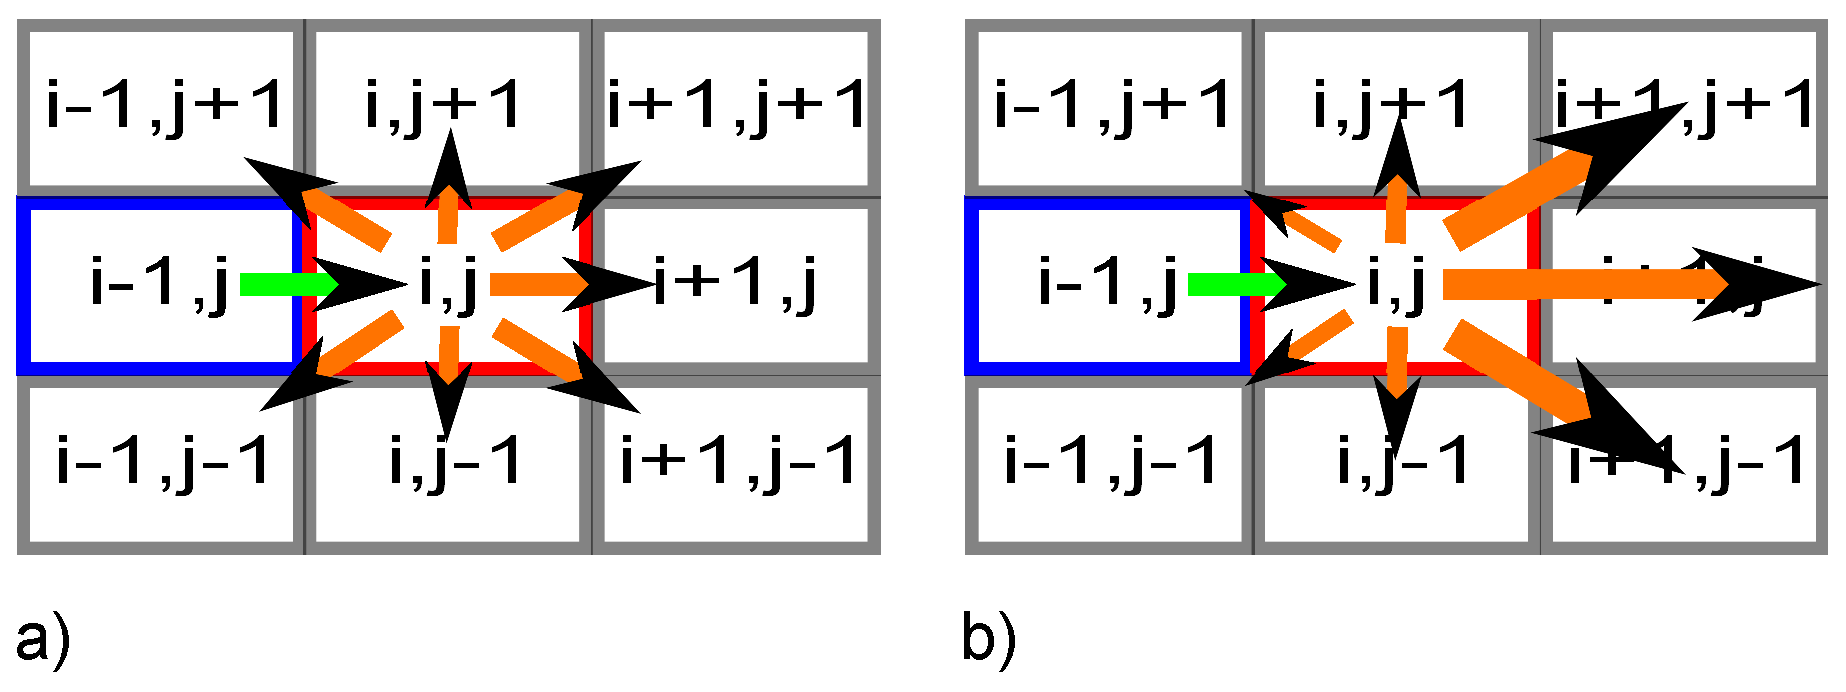
\includegraphics{weighting.eps}}
\caption{The available moves for a mesenchyme at $(i,j)$ after a epithelium at $(i-1,j)$ moves into its cell location. The probability that a move occurs is given by the length of the (orange) arrows. In a) the strength of discrimination against moves which are not aligned with the epithelium move is zero. In b) there is a high degree of discrimination against vectors of movement which are at angles to the movement vector of the epithelium.}\label{fig:arrows}
\end{figure} 



\subsection{Mesenchyme engulfment}\label{sec:engulfment}
Whereas in this cellular automaton it is possible for mesenchyme cells to become surrounded by epithelium, this is not observed in reality. In this section a mechanism is described which was implemented to try to reduce the frequency of this biologically-unrealistic occurrence in simulations.

'Engulfment' of a cell is the term I use to describe a situation where a mesenchyme is surrounded by a high number of epithelium cells. The number of surrounding epithelium cells above which a mesenchyme is deemed 'engulfed' is a parameter which I allow to be varied from a maximum of 8 (no possible engulfment), to zero (no nearest neighbours can be epithelium.)

There were two methods which were used to reduce the frequency of 'engulfment' of mesenchymes:

\begin{enumerate}
\item Disallow movement of mesenchyme cells to positions where they would be 'engulfed'.
\item Disallow movements of epithelium into cells which would result in situations where adjoining mesenchyme become engulfed (either directly or indirectly if a mesenchyme must be moved out of the way into a situation whereby it is surrounded by epithelium.)
\end{enumerate}

The implementation of this method (dependent on the threshold number of neighbouring epithelium cells which is chosen) could lead to a reduction in the occurrence of mesenchymal engulfment, although the magnitude of this decrease in frequency it should be said is not always visually evident. However, if a low threshold was applied (only a small number of neighbouring epithelium required before declaring a mesenchyme engulfed), biologically-infeasible patterns arose, where individual mesenchyme were surrounded by a layer of vacant space.

In summary I do not think this method is a particularly good choice for a biologically-realistic model of a UB which does not engulf mesenchyme cells. I also do not think that the rules which are described are reasonable as they assume a degree of sentience for the mesenchymes (where they 'look' to see if a move is allowed before making it), which is unrealistic.

\subsection{Non-local movement of mesenchyme}\label{sec:nonlocal}
It is observed that epithelium cells in the tip of a UB interact with an entire 'mass' of mesenchyme; eventually (via mutual interactions) resulting in a number of distinct mesenchyme subpopulations. With single occupancy of sites in a cellular automaton model, it is difficult to imagine how this type of behaviour could be recapitulated with local movement of mesenchymes out of the way of approaching epithelium. 

A possible solution to this would be to allow for multiple occupancy of sites by mesenchymal cells, although with multi-occupancy sites preferring to reduce their occupancy (by moving mesenchyme cells towards less densely-populated areas). This would require considerable work to accommodate these changes in the current model framework. It was suggested that this type of aggregate behaviour (where epithelium masses push on dense groups of mesenchyme) could be attained by allowing mesenchyme cells to be moved non-locally out of the way of encroaching epithelium. Although, this behaviour is less realistic than local movements, (as cells do not simply jump position), it can be thought of as representing the process whereby displacement of mesenchyme occurs via contact with epithelium, causing a movement of the entire mass. Since the mesenchyme cells are not heterogeneous in terms of their properties, in terms of the model, the movement of an individual cell non-locally to a position which is vacant is equivalent to a shuffling of the mesenchyme mass which results in an 'outer' mesenchyme occupying the same vacant position (assuming all other positions are the same between the two.) Furthermore, since the process causing the movement of the mass of mesenchyme is likely mechanical, its time scale can be thought of as faster than the general movement of cells; lending some justification for non-local jumping as representing movements which occur at a faster rate than cell movement or proliferation.

A schema which allows for non-local movement of mesenchyme cells is presented here. In defining which space of cells were available to a mesenchyme after it being encroached on by a epithelium cell, it is necessary to introduce the following concepts:

\begin{enumerate}
\item \textit{Principal axis} - the axis which is parallel to the direction of the movement vector of the epithelium as described in (\ref{eq:delta_move}).
\item \textit{Secondary axis} - the axis which is 'perpendicular' to the direction of the movement vector of epithelium.
\end{enumerate}

\begin{figure}[t] 
\centering
\scalebox{0.5} 
{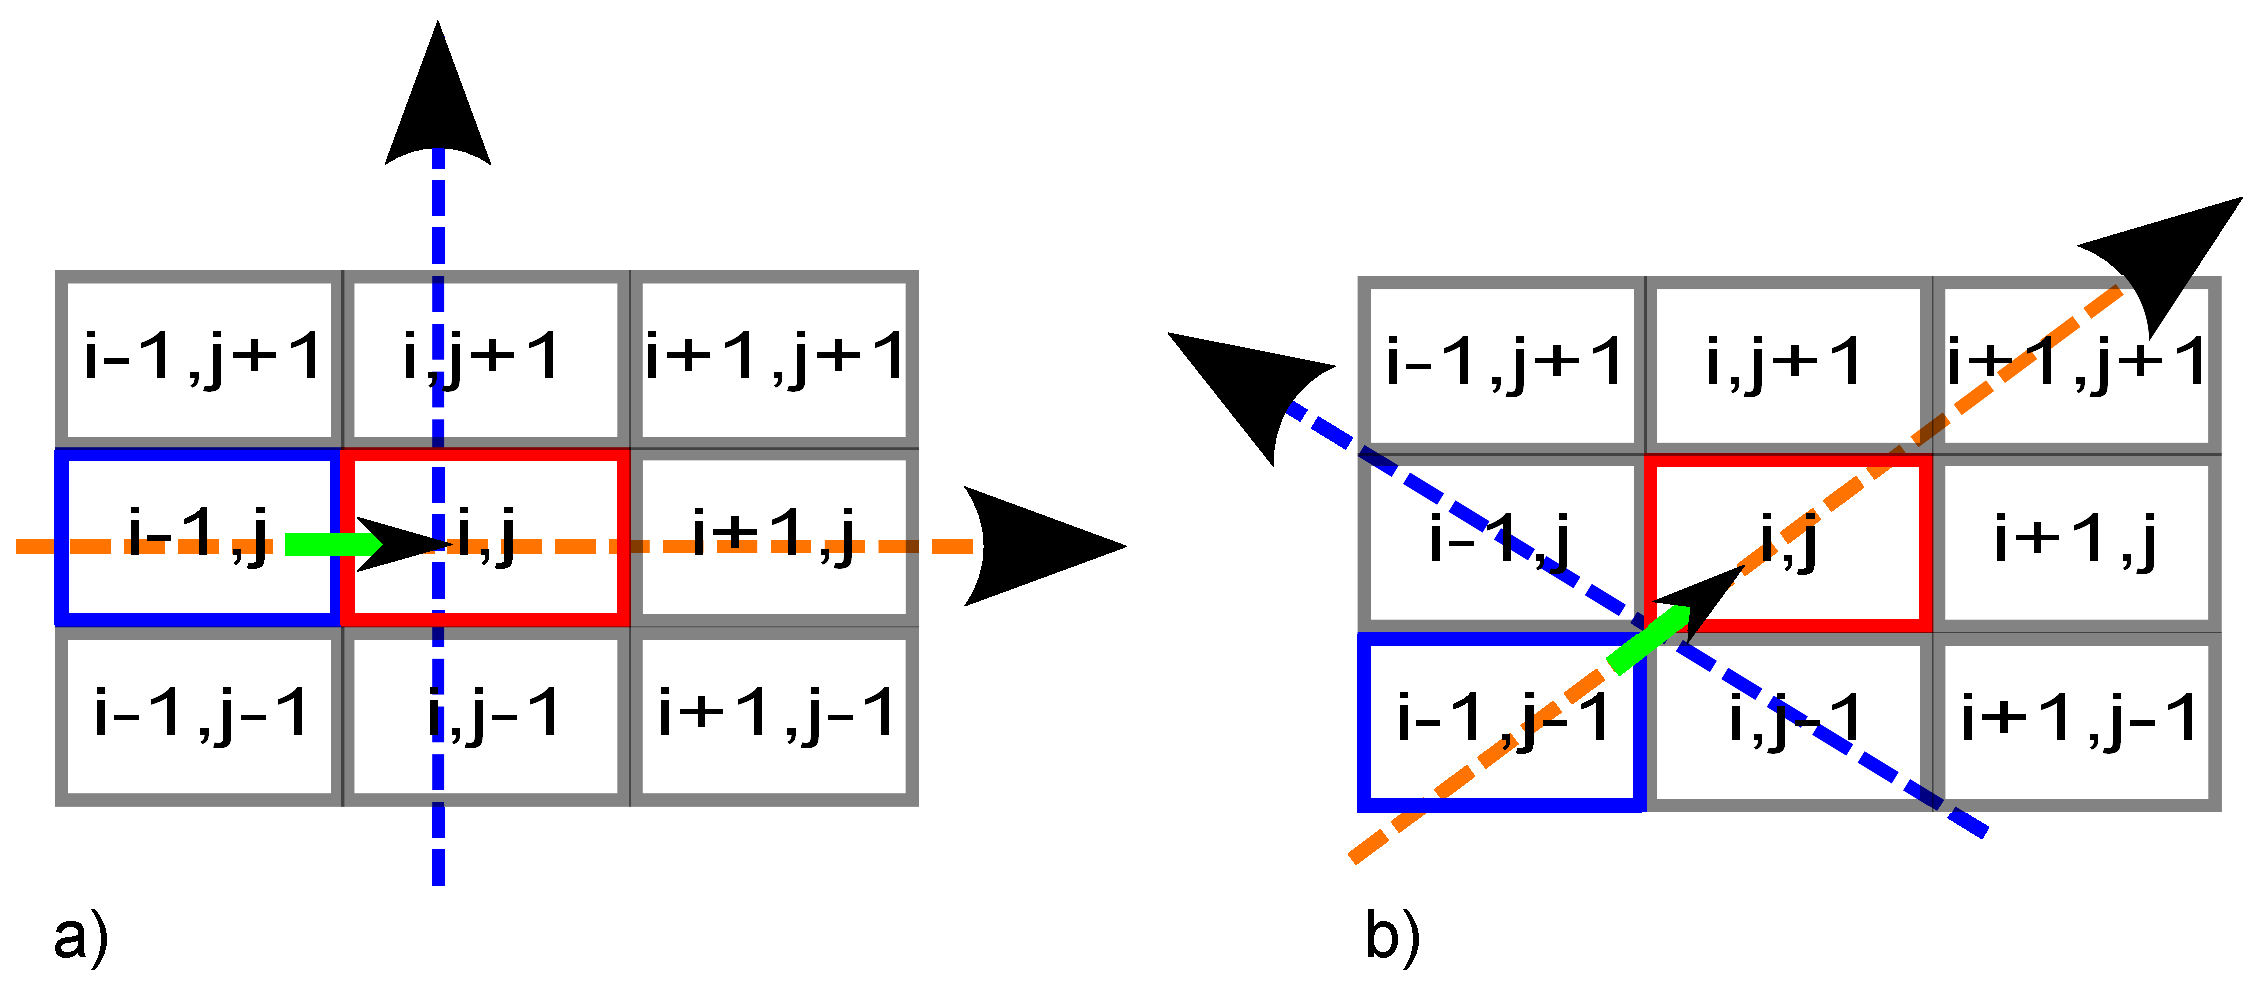
\includegraphics{axes.eps}}
\caption{The principal axis (in orange) and secondary axis (in blue) for two example movements. In a) the movement vector is horizontal, whereas in b) it is diagonal. The axes are not visually perpendicular in b) due to the fact that the cells are represented as rectangles rather than squares.}\label{fig:axes}
\end{figure} 

These two concepts are explained visually in figure \ref{fig:axes}. In defining these axes a rectangular space is traced out according to the maximum number of moves along the principal axis which are allowed, as well as the maximum number of moves sideways relative to the motion vector for the epithelium. The length of the rectangular space is chosen to start one unit behind (along the principal axis) the mesenchyme being considered, and ends after the maximum move length has been reached, $p}$; resulting in a length of $p + 2$. The width of the domain is given by specifying the maximum number of moves along the secondary axis which were allowed, $s$; resulting in a width of $2\times s + 1$. This allowed movement domain is shown in figure \ref{fig:rectangular}. 

\begin{figure}[t] 
\centering
\scalebox{0.5} 
{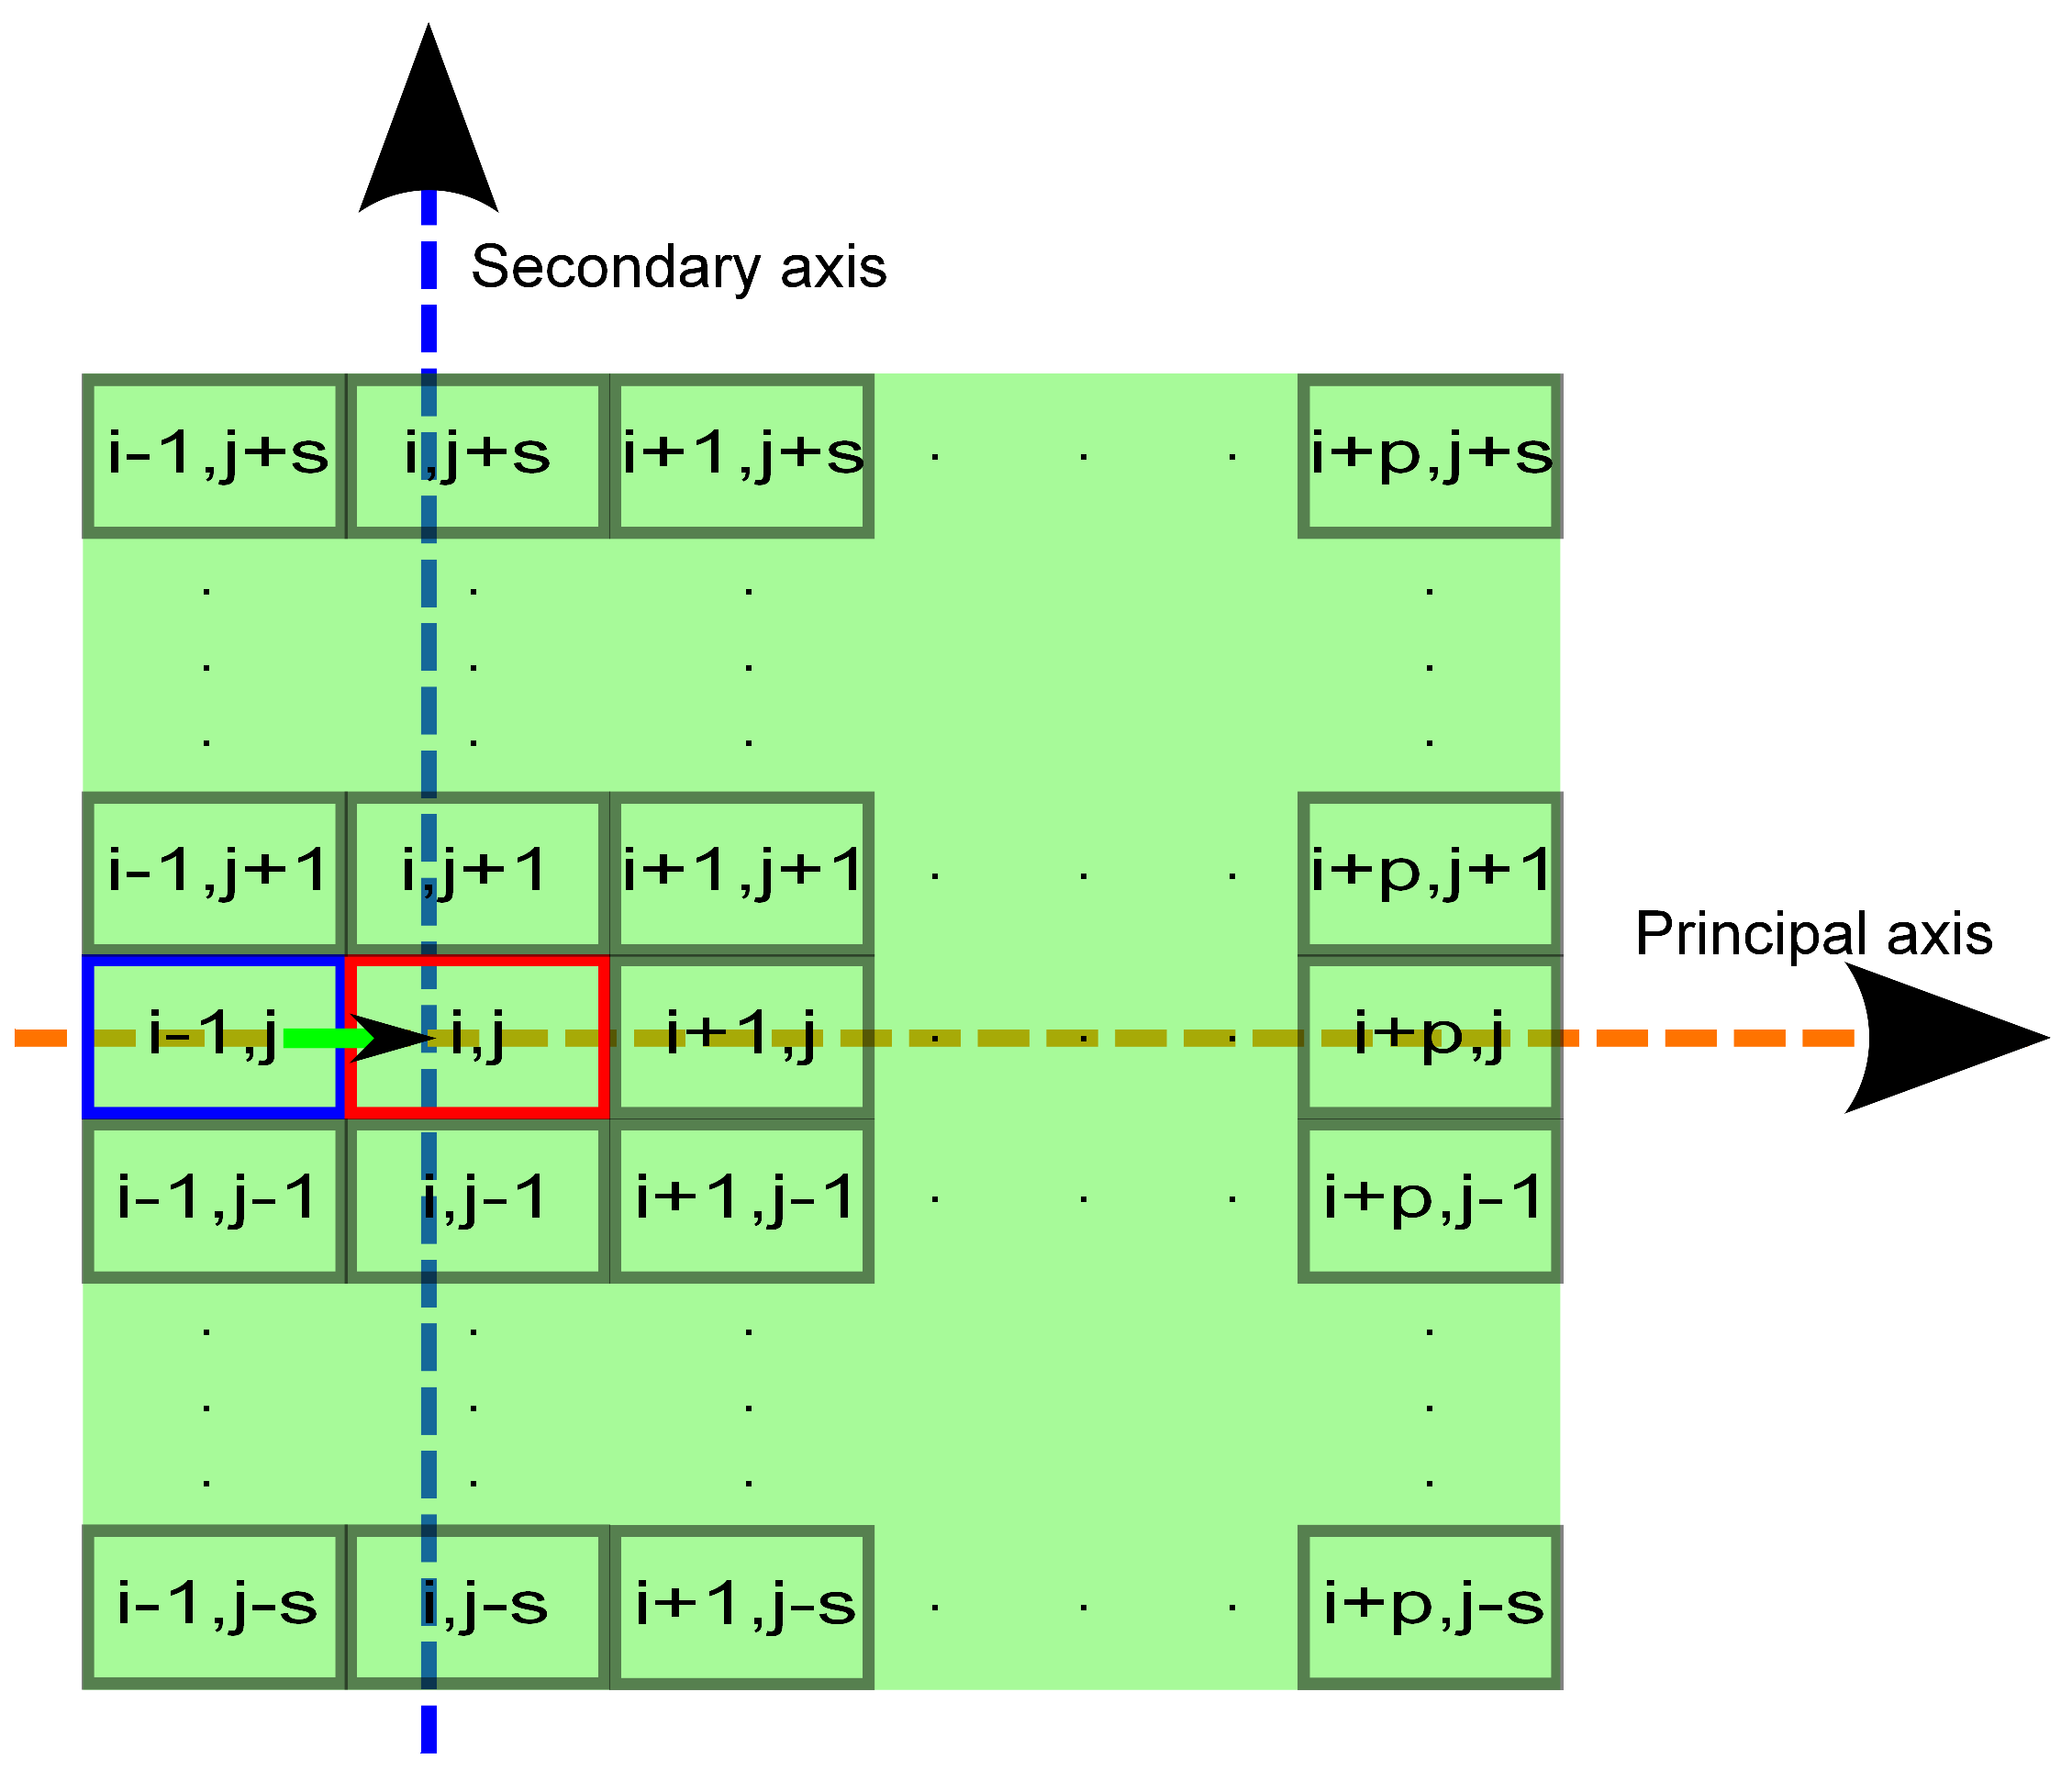
\includegraphics{rectangular.eps}}
\caption{The space (coloured green) of available moves for a mesenchyme at $(i,j)$ after a epithelium at $(i-1,j)$ moves into its cell location if non-local cell movement is allowed. Here $p$ and $s$ refer to the maximum allowed move distance forward and sideways respectively.}\label{fig:rectangular}
\end{figure} 

Currently, there is no bias towards any of the cells which lie in the rectangular domain of allowed moves. In reality it is more likely that moves will occur if they are at a small angle to the principal axis, and are closer to the current cell location. The former is dealt with heuristically by specifying a distance $s<<p$ to ensure that the movements of cells are, by majority at a small angle to the principal axis. The latter could potentially be dealt with by specifying a cost which depends on distance from the current cell. It would also be possible to allow a wider range of angular movements, with those movements resulting in the largest angle between the principal axis and the movement vector being discriminated against most strongly. However, both of these extra movement constraints require more parameters, and make the model more complex, with the possibility that they may not add much insight to the situation at hand. These may be revisited in the future however.

\section{Active movement of mesenchyme}
Up until this point the mesenchyme have been assumed to move only as a result of being 'pushed' out of the way by encroaching epithelium. Although this type of passive role for the mesenchyme could potentially be important for generating the branching pattern seen \textit{in vivo}, it would be insufficient to explain two stylized facts:

\begin{itemize}
\item The mesenchyme form a 'condensate' around the emerging UB tip. See figure \ref{fig:condensation}.
\item There are distinct lobes of mesenchyme cells expressing Six2 which surround the tips in each of the branches, with lower density regions in the 'stalk' region of epithelium. See figure \ref{fig:UB_branch} for a visual depiction of branching.
\end{itemize}

\begin{figure}[t] 
\centering
\scalebox{0.35} 
{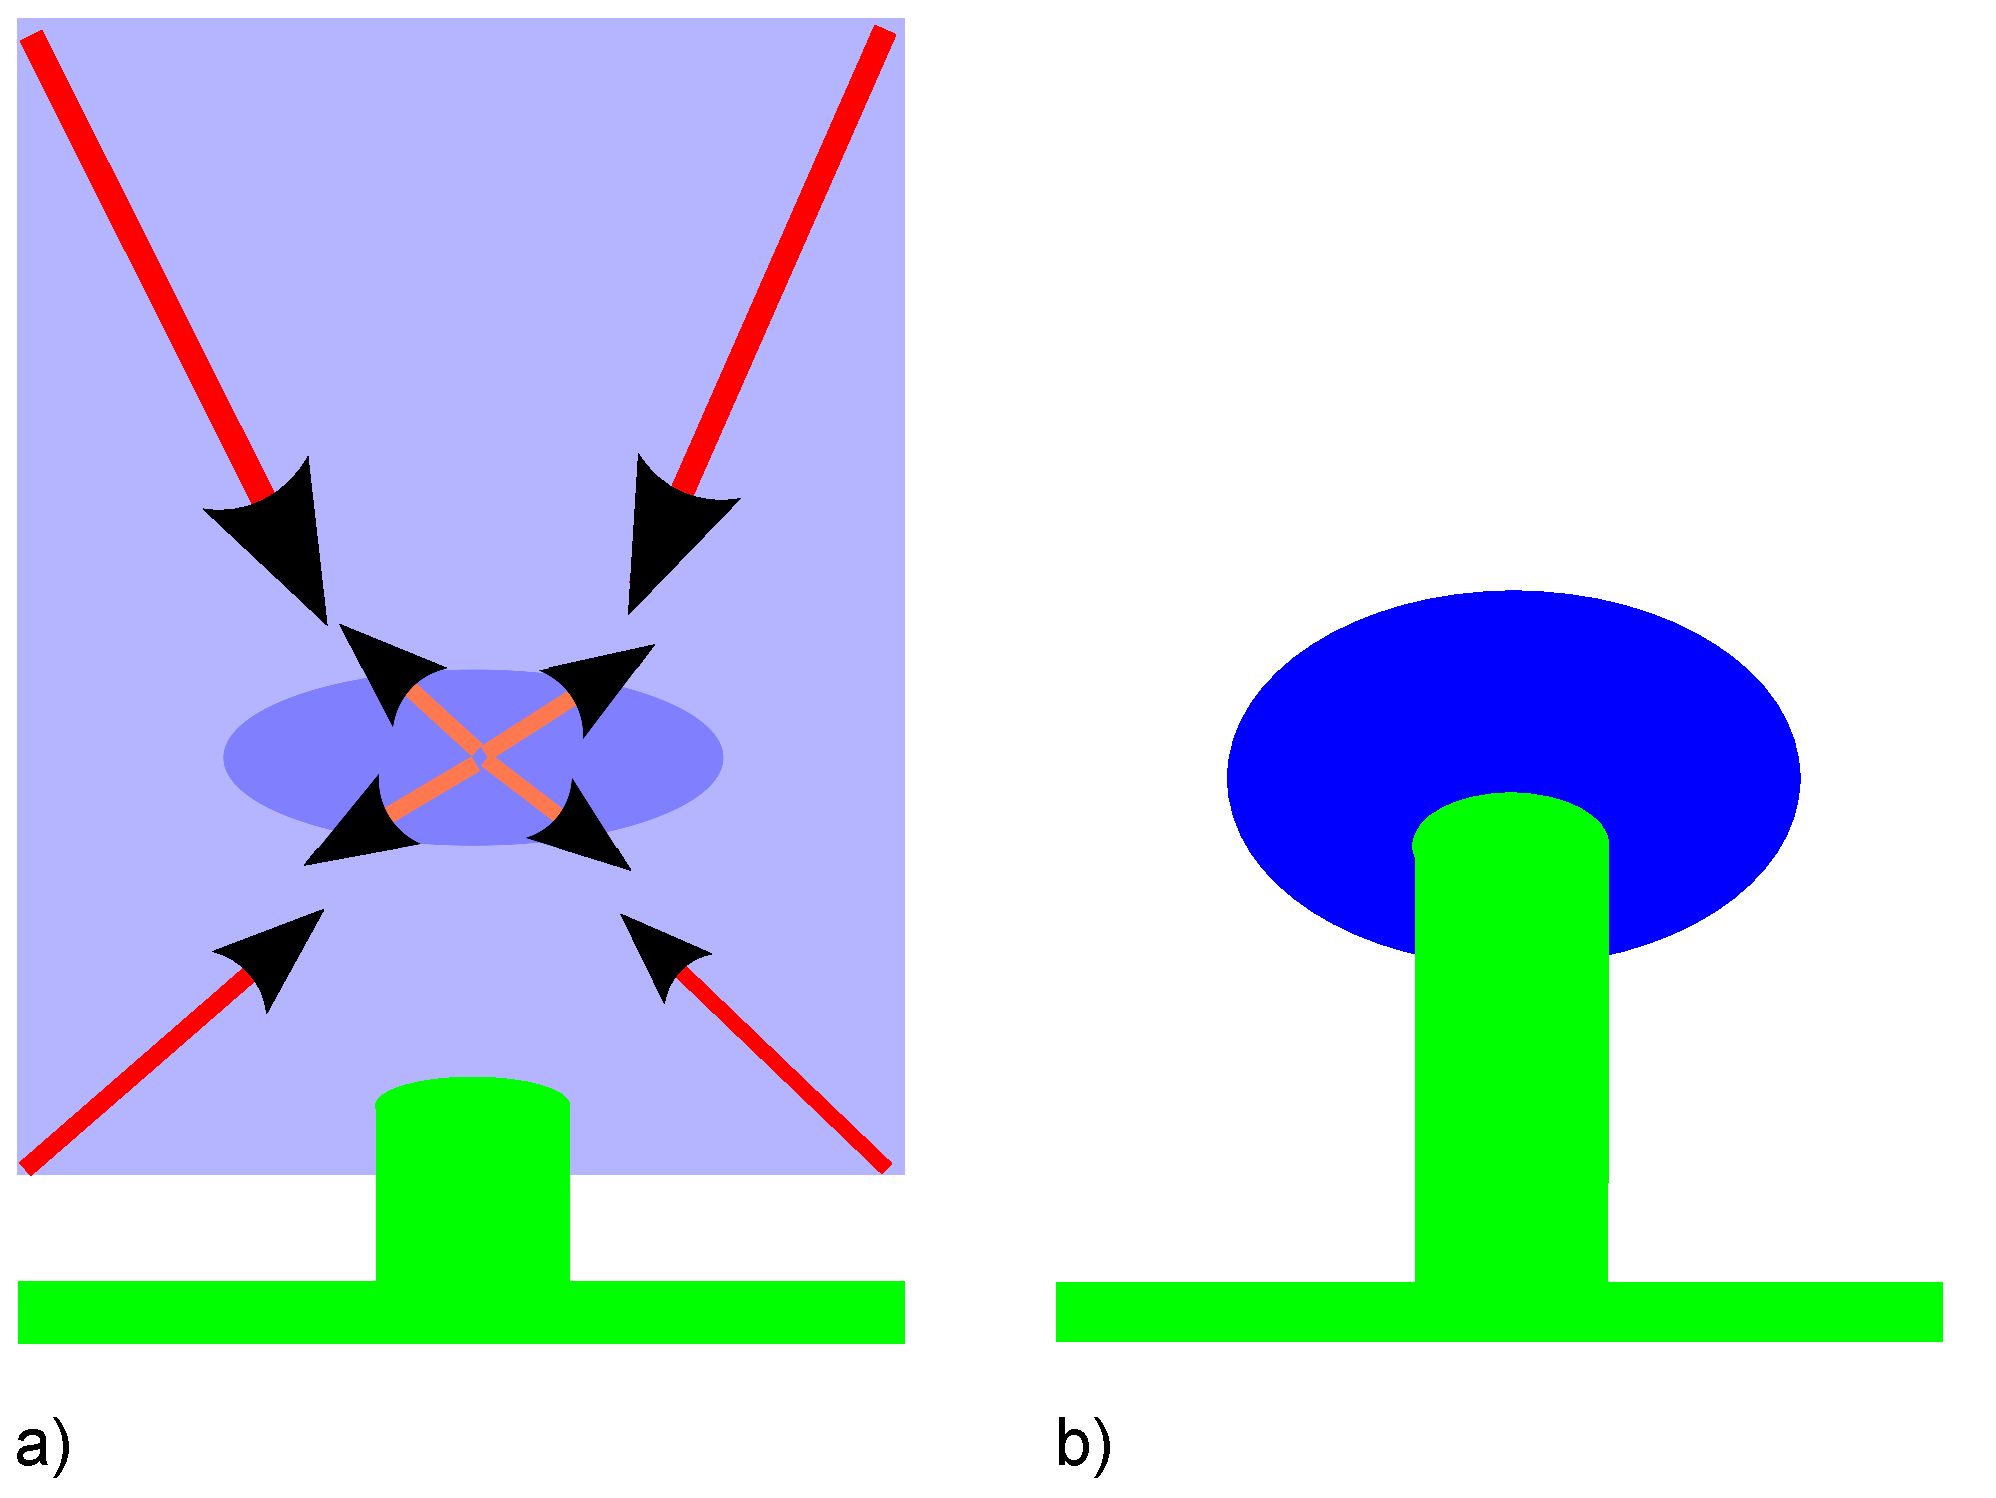
\includegraphics{condensation.eps}}
\caption{a) Shows the chemotactic (red arrows) and proliferative (orange arrows) potential mechanisms for the growth of a more dense mesenchyme cloud around the emergent UB tip. b) The finalised metanephric mesenchyme condensate around the grown UB tip.}\label{fig:condensation}
\end{figure} 

The condensation of mesenchyme likely occurs due in part to the growth of the UB bud into the MM; pushing any mesenchyme cells into a ring of mesenchyme which surrounds the tip. However, this mechanism is unlikely to explain why the number of mesenchyme cells increases throughout kidney development, and also that the mesenchyme (Six2 expressive) cells localise around the tips and not the stalks; although the latter point could be partially explained in continuum fluid models of the mesenchyme and epithelium, where the convective fluid flow fields result in eddies occurring behind the growing bud. Although there is little certainty as to what exactly causes the condensate to appear, it might be reasonably expected to be due to migration of mesenchyme towards the UB tip, as well as local proliferation of mesenchyme adjacent to the tip. The former could be due to a chemoattractive factor, whereas the latter could either be contact-mediated or paracrine in nature.

In the cellular automaton model presented here I allow both of the aforementioned methods to occur within the mesenchyme. I allow for chemoattraction of mesenchyme towards the UB, in a relationship which is weakened by distance, and a proliferative effect which is similarly affected by distance.

However, these two effects together are still insufficient to explain the formation of the discrete lobes of mesenchyme which ultimately form around distinct UB tips. In order to tackle this issue further assumptions and complexity are (unfortunately) needed, and I will postpone discussion of this until section \ref{sec:ret}.

\subsection{Chemoattraction of mesenchyme towards epithelium tips}\label{sec:activemesmove}
In order to allow for condensation of mesenchyme to occur due to its movement, I allow a mechanism which causes a movement of mesenchyme cells in a direction which is probabilistically weighted towards those cells which are closest to the epithelium. The pseudo-algorithm which is implemented here is of the form:

\begin{enumerate}
\item Calculate the probability that a move occurs. This can either be assumed to be location-independent, or negatively related to the distance of each of the target cells to the nearest epithelium.\label{point:mesactive}
\item Draw a pseudo-random $X\sim unif(0,1)$. If $X<P(move)$ then proceed to the next step. If not, then proceed to the next epithelium/mesenchyme in the simulation time step.
\item Find all the possible targets for the mesenchyme cell from the 8-nearest-neighbours which are currently vacant. 
\item Based on the rule chosen here implement one of the following:
\begin{itemize}
\item Assume a uniform probability of moving to each of available target cells.
\item Calculate probabilities which are weighted by the distance of each of the cells from the nearest epithelium. The method used here is to use a multinomial logistic distribution with a parameter specifying the extent of the strength of discrimination against moves which lead to more distant (from the epithelium) mesenchyme.\label{point:mesactive1}
\end{itemize}
\item Select one of the target moves by first creating intervals on [0,1] which correspond to each of the available targets, and comparing a pseudo-random $X\sim unif(0,1)$ with each of the intervals. If it coincides, then implement that corresponding move.
\end{enumerate}

Two mechanisms allow for the epithelium to influence the active moving behaviour of the mesenchyme. The first is that above in step \ref{point:mesactive}, which allows for the probability that a move occurs to be related to the inverse of the distance of each potential target cell from the epithelium. Whereas the first mechanism allows the probability of movement to dependent on distance, the second mechanism in \ref{point:mesactive1} directs the movement of the mesenchyme towards the nearest epithelium. This latter mechanism represents chemotaxis of mesenchyme towards the epithelium.

If chemotaxis occurs \textit{in natura} then it is likely driven by a chemoattractive factor which acts paracrinally. The epithelium would potentially produce the chemoattractant, which then diffuses in all directions (some of which are towards the mesenchyme). Presuming that the factor has more of an effect if it is in a higher concentration, this would then imply that the mesenchyme more distant from the epithelium are influenced less, and hence are less likely to move. However, if a move does occur the chemotaxis of the mesenchyme towards the epithelium would likely lead to a movement directed towards the epithelium. These aspects are represented phenomenologically by implementing both rules \ref{point:mesactive} and \ref{point:mesactive1}.

It is important to note that I have not assumed a particular form for the chemoattractant. Instead of creating a field for said factor, I proxy for it by, at each time step, calculating a distance matrix which represents the distance of each point in the array from the nearest epithelium. This calculation is done via dynamic programming for computational speed. The distance matrix is only updated once per time step however, as it is assumed that epithelium movements are not sufficiently significant as to change qualitatively the movement of the mesenchyme within a cell cycle time.

\begin{figure}[t] 
\centering
\scalebox{0.35} 
{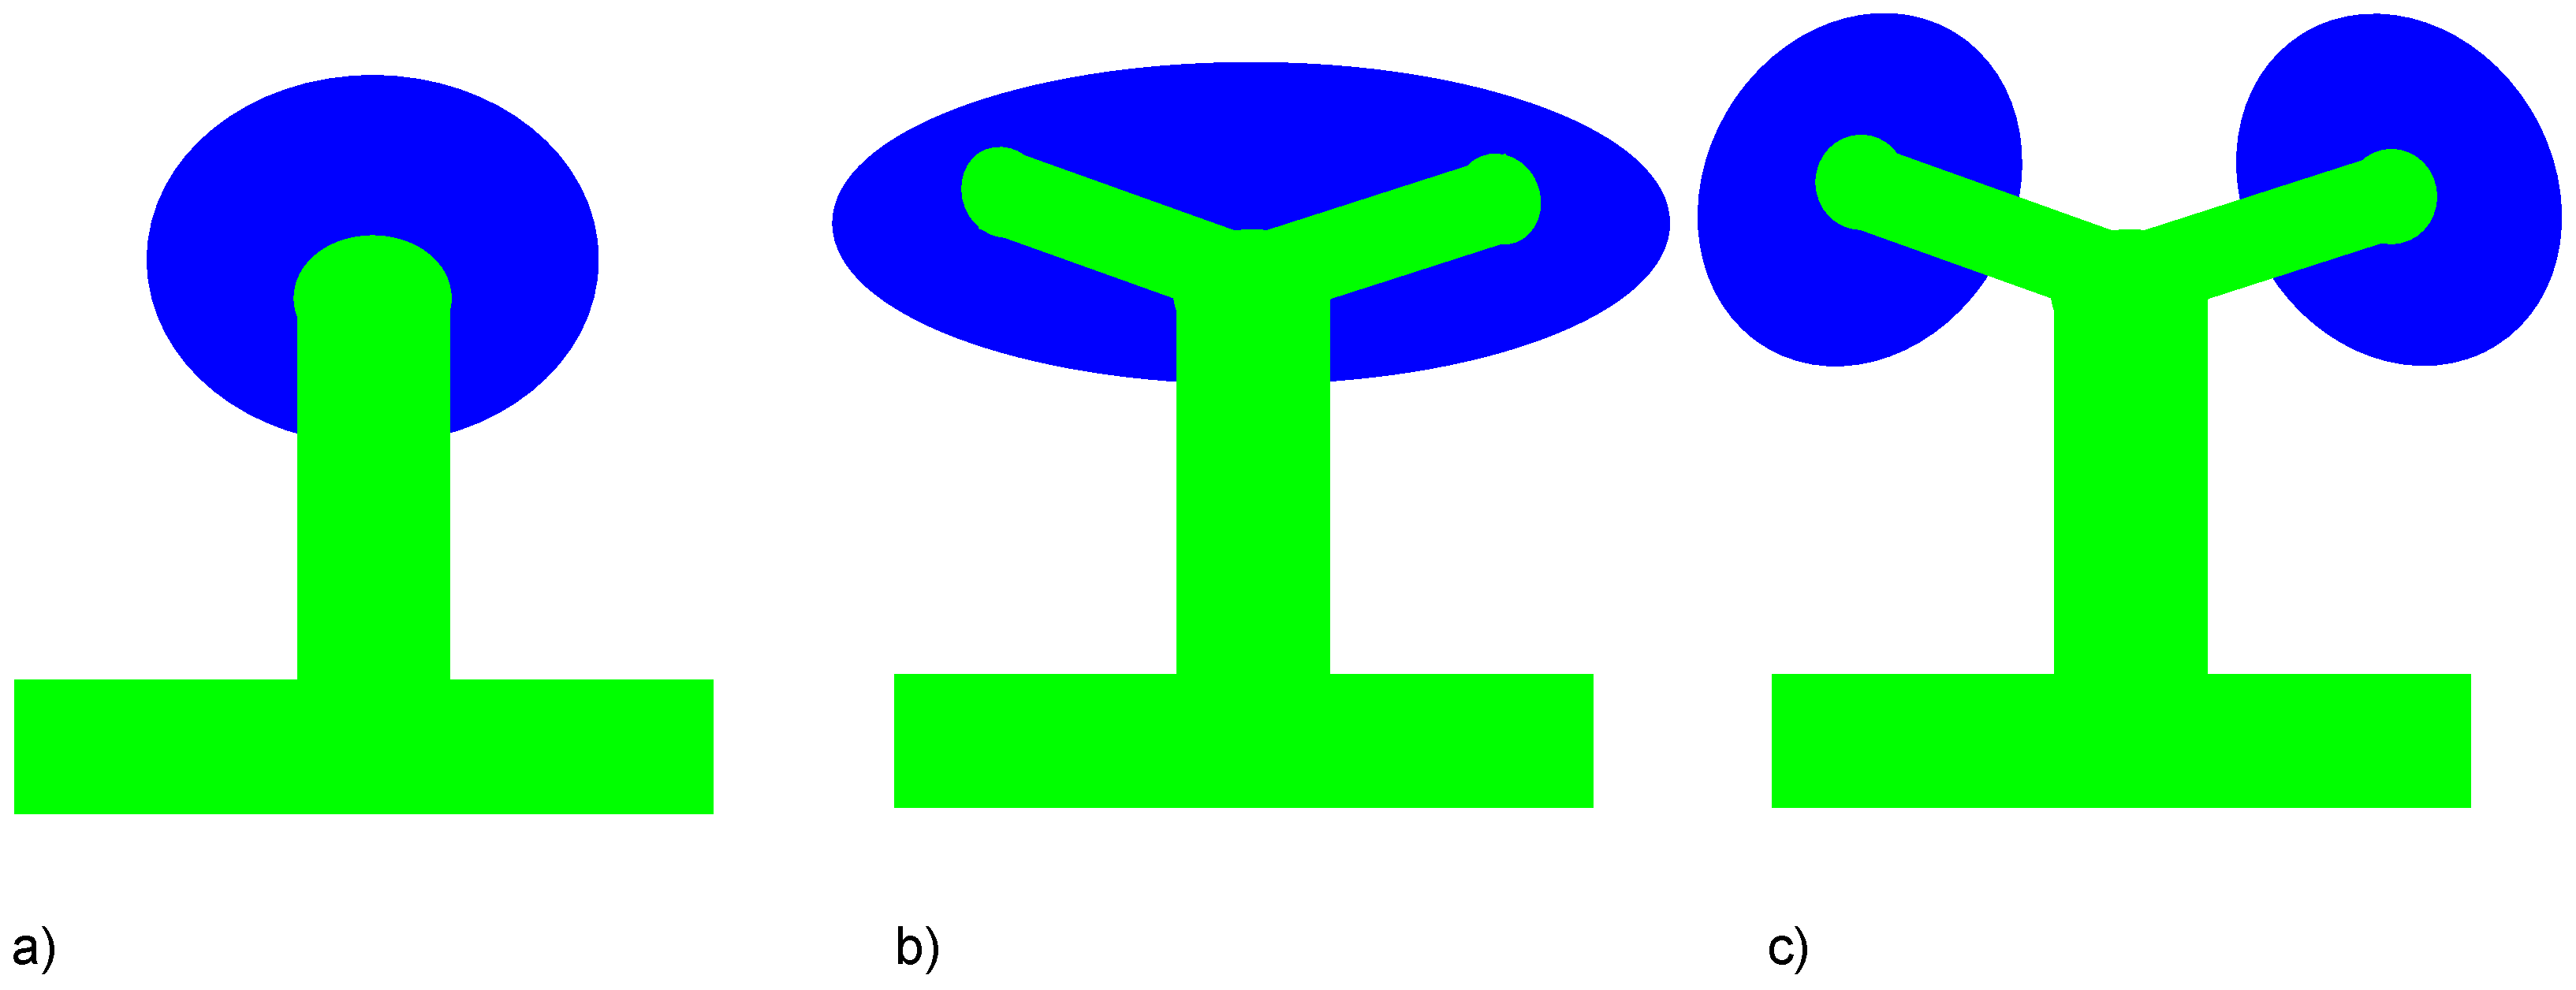
\includegraphics{UB_branch.eps}}
\caption{a) Shows the emergence of the UB bud. b) Shows the branching which occurs in the emerging bud. c) Shows the distinct lobes of mesenchyme which surround the tips of epithelium. In all diagrams the mesenchyme are coloured blue and the epithelium green.}\label{fig:UB_branch}
\end{figure} 


\subsection{Proliferation induced by proximity to epithelium}\label{sec:mesprolif}
The mechanism for proliferation is the same as that of the active mesenchyme movement, as detailed in section \ref{sec:activemesmove}, although now a new cell is either created or not opposed to just moved. Again, I allow for the possibility of two distinct schema for proliferation to occur. The first is that proliferation probability is positively influenced by the proximity of mesenchyme to epithelium. The other mechanism is to allow the probability of a target cell to be placed in a certain location to be positively influenced by the proximity of that cell to the epithelium.

\section{Heterogeneity in the epithelium: Ret-high and Ret-low cells}\label{sec:ret}
A qualitative feature which an adequate model of branching \textit{in vivo} should replicate is the discrete lobes of mesenchyme which aggregate around each individual epithelium tip. The biological/physical mechanism for this is currently not well understood. There are however, a number of inferences that could be made from the literature (and from a straightforward examination of the phenomenon itself). 

In order for discrete lobes of (Six2 expressive) mesenchyme to form solely around the tips, it is presumably the case that there is some heterogeneity between the niche at the tip as compared with the stalk regions. This is likely chemical, and could potentially be due to a difference in expression levels for a particular chemotactic/proliferative factor.

One potential feature that could be responsible for the differences between the tip and stalk niches is expression of Ret by the epithelium cells. It has been shown that epithelium cells compete with one another based on their expression levels of Ret to form part of the emergent UB (Chi et al. 2009). Furthermore the same authors go on to show that epithelium cells with high expression levels of Ret (as well as other proteins implicated in proliferation feed forward cycles), are present in the tips of the branches of the epithelium. This is not the case for the 'stalk' region of the epithelium trees which form. In the latter region there is a markedly lower level of Ret-expression. 

The authors initially propose that there could be four differences in properties between the Ret-high and Ret-low epithelium cells, which result in their differing geographical organisation. 

\begin{itemize}
\item Cell proliferation
\item Survival probability
\item Migration
\item Cell-to-cell adhesion
\end{itemize}

The authors find little evidence of differences in proliferation between the Ret-high and Ret-low epithelium; casting doubt on the first mechanism. Similarly, they find no heterogeneity in cell apoptosis between the two types of cells. Although the authors only search for the presence of a particular (yet important) marker of cell-cell adhesion, beta-cadherin, they nonetheless find no evidence for differences in its expression between the epithelium cells at the tip and in the stalk. They do however find evidence that cell-cell competition is an important mechanism for the emergence of the initial bud, as well as the elevated prevalence of Ret-high cells in the tips. Although the biological basis of this competition is not understood, its relative winners (those cells nearest the tips) are found to be those cells which are Ret-high. As such as a first approximation I allow there to be two distinct epithelium cell types: Ret-high, and Ret-low. Both these cells are attracted to sources of GDNF, although the former are more strongly so. Note, it needn't be the magnitude of the attraction to GDNF sources which results in the differential movement of Ret-high and Ret-low cells towards the tips. However, this as a first approximation will allow for the recapitulation of the features seen in practice. Another point of note is that likely the level of Ret-expression could be perhaps be more realistically modelled by allowing cells to exist on a spectrum of Ret-level; however, as the experimental literature seems to focus on binary descriptions of cells: Ret-high and Ret-low; it is believed that this approximation is perhaps not too over-simplifying. 

However, just having two types of cell which are differentially attracted to sources of GDNF is insufficient to create the distinct lobes of mesenchyme around tips. In order for this to be the case there needs to be some difference in the way in which mesenchyme are influenced by the two cell types. This could be because the Ret-high cells are relatively more attractive to the mesenchyme, or cause greater proliferation rates for the adjacent mesenchyme, or a combination of these two features (since mesenchyme apoptosis is not thought to be an important mechanism for kidney morphogenesis).

As a first approximation I assume that the mesenchyme are attracted towards and interact \textit{only} with the Ret-high cells. This could be an over-simplification, as the mesenchyme may interact with both types of Ret-expressing epithelium cells. As such, at each time step, I calculate the distance of the mesenchyme to the nearest Ret-high epithelium cell, and then use the rules detailed in sections \ref{sec:activemesmove} and \ref{sec:mesprolif}. In order to allow for the fate of epithelium cells to be endogenously determined in the system, I also allow for transformation of Ret-low to Ret-high cells, and vice versa. The details behind this mechanism are included in section \ref{sec:rettransform}. In order to allow for movement of epithelium cells of different Ret-expression levels in the epithelium layer (up until now disallowed since there are no vacant spots for the cells to move into), I also implement a new method which I term 'competing'; where epithelium cells compete with one another to get closer to sources of GDNF, with the Ret-high being more 'competitive' than Ret-low cells. The details behind this method are explained in section \ref{sec:retcompetition}.

\subsection{Transformation of Ret-expression level in epithelium}\label{sec:rettransform}
It is known that there is an intrinsic heterogeneity in Ret-activity in epithelium cells within the Wolffian Duct. However, what is not known is whether cells' fates are determined at their birth, or whether they maintain a degree of pluripotency throughout their lifetimes. As there is considerable uncertainty surrounding whether it is possible for an epithelium cell to transition from being a Ret-low to Ret-high cell, and vice versa, I allow for five distinct rules which are thought to encapsulate a wide variety of possible mechanisms. In all cases below I assume that daughter cells of epithelium are created in exact likeness to their parents (in terms of Ret-activity). This may not be case \textit{in vivo}, but by allowing cells to transition from one type to another based on biological conditions, it is believed that this assumption is not as restrictive as it might first appear.

\begin{enumerate}
\item \textit{No transformation of epithelium cells} - epithelium cells cannot transition from one type to another.
\item \textit{Ret-low to Ret-high transitions at arbitrary rate} - epithelium cells are allowed to transform from low to high type, but cannot move back the opposite direction. The probability of a transition is determined by the user and is independent of biological conditions.
\item \textit{Ret-low to Ret-high and vice versa transitions, each with own arbitrary rate} - Same as above, but now allow for reversible transition. The probabilities of transitions are determined by the user and is independent of biological conditions.
\item \textit{Ret-low to Ret-high transitions at a rate which is determined by local GDNF concentration} - probability of transitions here is determined by a function (with its user-specified parameters) of local GDNF concentration.
\item \textit{Ret-low to Ret-high and vice versa transitions at a rate which is determined by local GDNF concentration} - same as above, but allow for reverse transition.
\end{enumerate}

The rules above which allow for transition from one cell type to another based on GDNF are assumed to have associated probabilities which are given by the following function:

\begin{equation}\label{eq:transition}
P(transition)= \Phi (C1 + C2\times GDNF)
\end{equation}

Where in (\ref{eq:transition}), $\Phi$ refers to the cumulative probability distribution for a standard normal. The reason for allowing the rate of Ret-low to Ret-high transitions to be determined by GDNF concentration is that \textit{in vivo}, Ret-high cells are found at the tips of branches, where GDNF is assumed to be relatively high. Whilst it is not necessarily the case that GDNF is the factor which determines Ret-fate of epithelium cells, it is assumed here as a first approximation aimed at recapitulating the patterns of gene expression seen \textit{in vivo}. In the last rule, where both directions of transition are allowed, the simulation allows for different $C1$ and $C2$ for each direction. This allows for the possibility that GDNF to have different effects on the determination of rate for the forwards (Ret-low to Ret-high) and backwards directions. This is an assumption which is aimed at recapitulating two stylised facts of UB branching: firstly Ret-high cells are found at UB tips; secondly, Ret-low cells are found in the stalk regions. 

\subsection{Ret-contingent competition}\label{sec:retcompetition}
Competition amongst epithelium cells on the basis of Ret-expression level has been shown to be part of a realistic description of initial Uretic Bud formation; with the bud being made predominantly of cells which are Ret-high. At current the model does not allow for movement of epithelium cells if there are no adjacent vacant cells. This is a consequence mainly of the model's cellular automaton formulation, rather than representing a biologically-realistic description where epithelium cells continually move around in the epithelium layer. Since, up until this point there was no heterogeneity in the epithelium cells, there was no need to consider mechanisms for allowing this type of movement. However, in order to allow for epithelium cells to 'compete' to become part of the emergent UB, this motivated the introduction of a new behaviour (I term competing), which can occur as well as moving and proliferating. The definition I give 'competing' is when two Ret-different cells in the epithelium layer swap places (the Ret-high probabilistically taking the position with the highest GDNF).

The decision as to whether to move down the algorithmic path corresponding to 'competing' is determined at the same stage as that governing moving and proliferating. After a decision has been made to go down the competing path, it is still not determined whether competition will take place. Firstly, I assume (I believe without loss of generality) that Ret-high cells are the active movers; in other words, it is these types of cells which initiate and ultimately go through competition. Secondly, it is assumed that a Ret-high cell can only swap positions with a Ret-low cell if there is one adjacent, and that the concentration of GDNF in at least one of the target cells is higher than the current position GDNF concentration. This latter stipulation is so that Ret-high cells only swap with Ret-low cells if there is additional GDNF concentration to be gained by the move. If the aforementioned conditions are satisfied, then the simulation allows competition (swapping) to take place probabilistically. In order to allow for a migration of Ret-high cells towards tip areas, I calculate a probability which is a positive function of the GDNF gradient between the neighbouring Ret-low cell with the highest GDNF concentration, and the current cell position. As a simplifying approximation, I also allow swaps to take place only with the nearest Ret-low cell with the highest GDNF concentration. Although epithelium cells likely do not move as directly towards sources of GDNF as this, it is not believed that this assumption will affect the overall simulation results (although should reduce computational time).

\section{Cell death}
The current version of the simulation does not allow cell death directly; only indirectly through the epithelium's ability to (dependent on the exact rules implemented) 'overtake' a position currently occupied by the mesenchyme. Later versions will allow the user to stipulate differing death rates for the epithelium and mesenchyme, and also allow these to be context-dependent (dependent on, for example, the connectivity of the cell in question).

\section{Creation of the epithelium layer}
Two different schema are considered for the creation of an epithelium layer:
\begin{itemize}
\item A flat layer of epithelium at the base of the simulation domain to emulate \textit{in vivo} formation of the initial Uretic Bud. Although this layer is \textit{in rerum natura} mono-layered, I choose to use a multi-layered epithelium. This is to allow for the fact that the simulation domain is two dimensional whereas in practice it is three dimensional. Making the layer multi-layered allows cells which are outside of the simulation plane to pass into the layer bordering on the ECM/mesenchyme.
\item A randomised mass of epithelium cells towards middle of the simulation domain representing \textit{in vitro} experimental conditions. The idea here is that branching arises partly as a result of local depletion of GDNF concentration in 'crypts' of epithelium next to outgrowths.
\end{itemize}

\section{Branching measurement and visualisation}
\subsection{Perimeter-to-area ratio vs circle}
A circle is the 2 dimensional object which has the lowest perimeter-to-area ratio (or put another way, it maximises area for a given perimeter). An object which is highly branched will, by contrast, have a relatively high ratio of perimeter-to-area. Hence, by comparing the perimeter-to-area ratio from the mass of epithelium with that of a circle with the same number of cells (the measure of area in the CA), the latter having a ratio of $ratio = \frac{2}{r}}$, this could be taken to be a reasonable measure of the level of branching in the epithelium mass. However, it should be noted that this isn't necessarily a measure of branching, and could just be a measure of the fractal nature of the mass, without \emph{per se} having distinct branches.

It is difficult to exactly calculate the perimeter of a contiguous mass of epithelium cells in this cellular automaton model, since this would involve coding the specific define characteristics of a cell on the edge of the mass. Instead of calculating the perimeter exactly, I borrow from medical imaging segmentation, using the Matlab function \emph{bwconncomp} to calculate an approximate measure of the perimeter. This same functionality also yields an approximate area, which was compared to the exact area (simply the number of epithelium cells), and found to be in good correspondence. Visually the approximate perimeter also appeared to follow that seen, but further work here is needed to confirm that the approximate method here is reasonable (note to Ben: an idea - calculate the gradient of the image in both x and y and threshold it. All the perimeter cells should be connected. Then just use bwconncomp on the thresholded image. You can use the latter to calculate get the pixel ids.)

\subsection{Medial axis skeleton branching}\label{sec:branches}
Another method to investigate branching in topology is to find the medial axis skeleton of the closed curve representing the perimeter of the object. The medial axis (in two dimensions) is the locus of points within the object which have two (or more) nearest points on the edge of the image. This means that a circle drawn with its centre at a particular point on the locus, will be tangent to the perimeter contour at two or more places. Example of medial axis skeletons are shown in figure \ref{fig:medial} for an ellipse and an arbitrary perimeter.

Luckily Matlab has already a built-in function, \emph{bwmorph}, which estimates the medial axis skeleton of an object, and also allows the user to extract the number of implied branch points from the skeleton. The visualisation of the estimated medial axis skeleton along with the number of branch points appears to be a nice way to estimate the degree of branching occurring within the epithelium mass. The latter was normalised by the area of the figure, as this appeared to be a better method of discriminating between whether an object was spherical vs branched.

\begin{figure}[t] 
\centering
\scalebox{0.5} 
{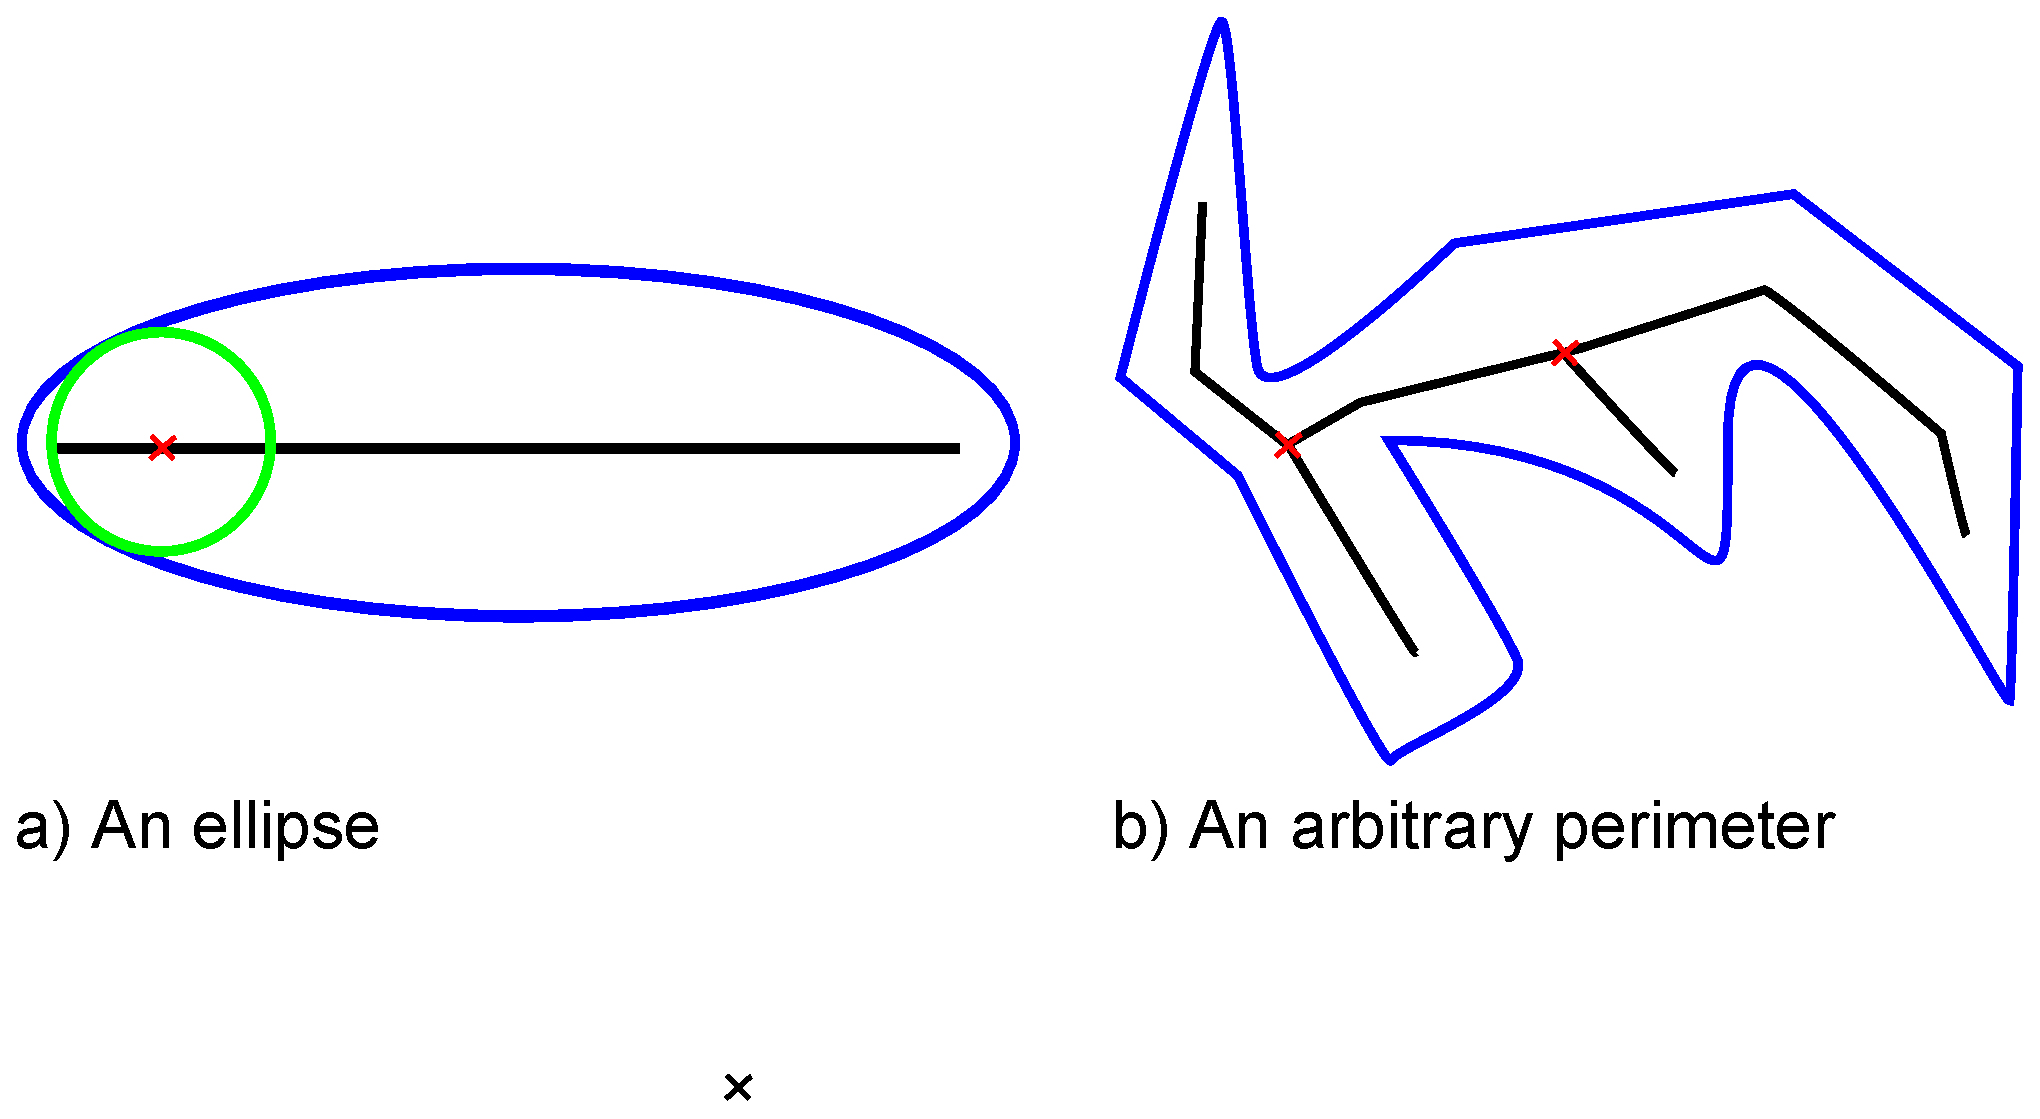
\includegraphics{medial.eps}}
\caption{The medial axis skeleton (in black) for a) an  ellipse and b) an arbitrary perimeter. In a) the red cross shows the centre of the green circle (which is tangent to the perimeter at two points.) In b) the red crosses show branch points in the medial axis skeleton.}\label{fig:medial}
\end{figure} 


\end{document}